\chapter{Introduction}

\section{Flow in Magnetic Mirror Configuration}
Plasma flow in magnetic mirror configurations have been studied extensively in plasma physics due to its frequent precense in many areas such as the accretion flow \cite{jockers_stability_1968,aikawa_stability_1979}, and magnetic nozzle\cite{smolyakov_quasineutral_2021}. However, the stability of these configurations remains a debatable subject.

The flow in magnetic nozzle an example of flow in magnetic mirror configuration. The magnetic nozzle is a convergent-divergent magnetic field that guides, expands and accelerates a plasma jet into vacuum for the purpose of space propulsion. \cite{andersen_continuous_1969,boswell_experimental_2004,williams_fusion_2003} The magnetic field in the magnetic nozzle plays a similar role to the walls of a Laval nozzle, see Fig. \ref{fig:magnetic-nozzle}. The curvature of magnetic field confines and accelerates the charged particles. The plasma flow starts from subsonic at one end and accelerated to supersonic speed at the exit. Although magnetic nozzle has been studied extensively, its stability remains a topic of active research.

\begin{figure}[h]
	\centering
	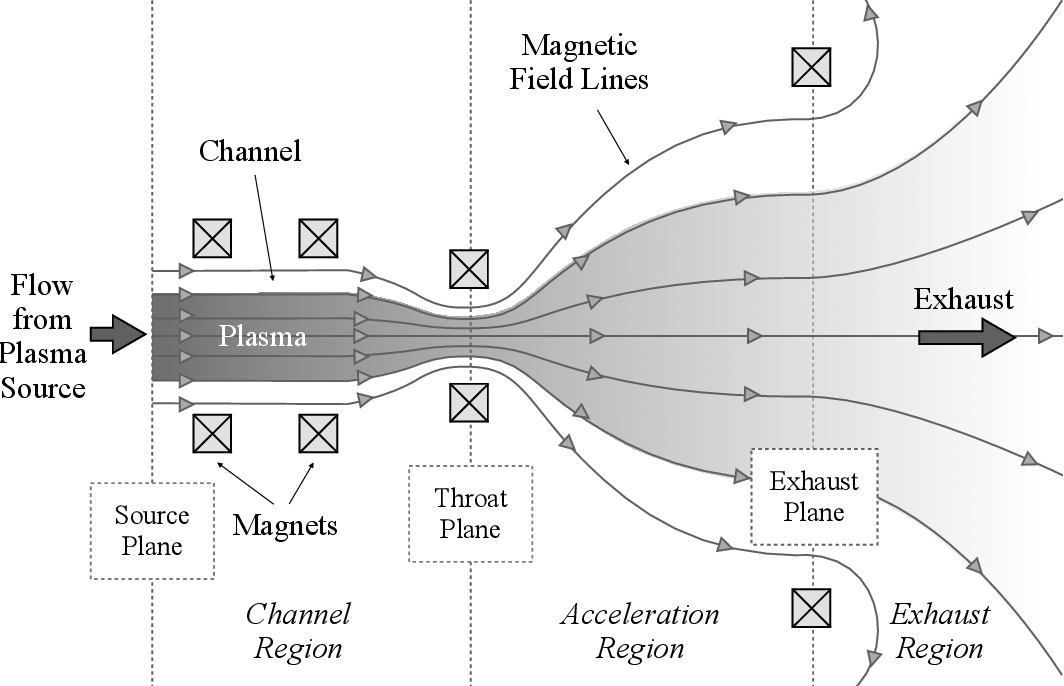
\includegraphics[width=0.7\linewidth]{img/introduction/magnetic_nozzle}
	\caption{Example of a magnetic nozzle configuration. In our models, we define the magnetic nozzle as the region downstream from the throat plane, which can be further divided into an acceleration region and exhaust region. The channel connects the plasma source (not shown) with the magnetic nozzle. \cite{little_performance_2015}}
	\label{fig:magnetic-nozzle}
\end{figure}

Accretion flow is another example of flow in magnetic mirror configuration. It is similar to that in magnetic nozzle. The plasma flow is at rest at infinity and accelerated towards the steller object due to gravity. It is natural to compare the study of its instabilities to that of magnetic nozzle due to the similarity of the two system. However, the results are still debatable. \cite{keto_stability_2020,aikawa_stability_1979,stellingwerf_stability_1978}

\section{Goal of this Thesis}
The goal of this thesis is to study the instabilities of the magnetic mirror configuration given certain boundary conditions and equilibrium velocity profiles.

To achieve the goal, first we need to study the spectral method for solving the instability problem. To use spectral method, it is necessary to understand different discretizations of the operators, such as finite difference, finite element and spectral element method.

Once the spectral method is introduced, we can use it to study the instability of plasma flow in magnetic nozzle as an eigenvalue problem. We can obtain results by using different discretization techniques. By comparing the results from different approach, we can increase the credibility of the true solution.

However, spectral method is not suitable when the equilibrium velocity profile is transonic due to the precense of singularity at the sonic point. We need to solve the singular perturbation problem around the singularity analytically. Then starting from the singular point, we can use shooting method to find eigenvalues.

\section{Outline of the thesis}
The thesis will be divided into several chapters. In chapter 2, spectral method will be introduced. Chapter 3 will focus on the physics of flow in magnetic mirror configuration and derive the governing equations for charged particles, the linearized equations of motions. Following this, we will analyze the problem analytically in chapter 4. Moving to chapter 5, numerical experiments will be conducted. The conclusion will be made in chapter 6.
